        \documentclass{standalone}
        \usepackage{tikz}
        \usetikzlibrary{arrows}
        \usepackage{amsmath}
        \usepackage{amsfonts}
        \begin{document}
        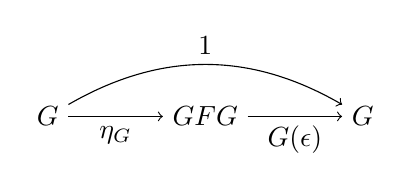
\begin{tikzpicture}

    \node at (0,0) (G1) {$G$};
    \node at (2,0) (GFG) {$GFG$};
    \node at (4,0) (G2) {$G$};
    \draw[->] (G1) -- node[below] {$\eta_G$} (GFG);
    \draw[->] (GFG) -- node[below] {$G(\epsilon)$} (G2);
    \draw[->] (G1) to [out=30,in=150] node[above] {$1$} (G2);
        \end{tikzpicture}
        \end{document}
